\documentclass[12pt,letterpaper]{article}
\usepackage{fullpage}
\usepackage[top=2cm, bottom=4.5cm, left=2.5cm, right=2.5cm]{geometry}
\usepackage{amsmath,amsthm,amsfonts,amssymb,amscd}
\usepackage{lastpage}
\usepackage{enumerate}
\usepackage{fancyhdr}
\usepackage{mathrsfs}
\usepackage{xcolor}
\usepackage{subfig}
%\usepackage{biblatex}
\usepackage{graphicx}
\usepackage{listings}
\usepackage{hyperref}
\usepackage[compat=1.1.0]{tikz-feynman}
\newcommand{\avg}[1]{\big<#1\big>}

\hypersetup{%
  colorlinks=true,
  linkcolor=blue,
  linkbordercolor={0 0 1}
}
 
\renewcommand\lstlistingname{Algorithm}
\renewcommand\lstlistlistingname{Algorithms}
\def\lstlistingautorefname{Alg.}

\lstdefinestyle{Python}{
    language        = Python,
    frame           = lines, 
    basicstyle      = \footnotesize,
    keywordstyle    = \color{blue},
    stringstyle     = \color{green},
    commentstyle    = \color{red}\ttfamily
}

\setlength{\parindent}{0.0in}
\setlength{\parskip}{0.05in}

% Edit these as appropriate
\newcommand\course{FYS5555 }
\newcommand\hwnumber{1}                  
\newcommand\Name{Federico Nardi}           


\pagestyle{fancyplain}
\headheight 35pt
\lhead{\Name}
             
\chead{\textbf{\Large \course  - Project \hwnumber}}
\rhead{\today}
\lfoot{}
\cfoot{}
\rfoot{\small\thepage}
\headsep 1.5em

\begin{document}

\section{Feynman rules}
The lowest order diagrams for the process $\mu^- \mu^+ \rightarrow b\, \bar{b}$ are the following

\begin{figure}[!h]
\subfloat[]{
	\feynmandiagram [horizontal=a to b] {
	  i1 [particle=\(\mu^{-}\)] -- [fermion, momentum =\(p\)] a -- [fermion, rmomentum=\(k\)] i2 [particle=\(\mu^{+}\)],
  	a -- [photon, edge label=\(\gamma\), momentum'=\(q\)] b,
  	f1 [particle=\(\bar{b}\)] -- [fermion, rmomentum'=\(p'\)] b -- [fermion, momentum' =\(k'\)] f2 [particle=\(b\)],
	};
}\qquad
\subfloat[]{
	\feynmandiagram [horizontal=a to b] {
	  i1 [particle=\(\mu^{-}\)] -- [fermion, momentum =\(p\)] a -- [fermion, rmomentum=\(k\)] i2 [particle=\(\mu^{+}\)],
  	a -- [photon, edge label=\(Z\)] b,
  	f1 [particle=\(\bar{b}\)] -- [fermion, rmomentum' =\(p'\)] b -- [fermion, momentum' =\(k'\)] f2 [particle=\(b\)],
	};
}\qquad
\subfloat[]{
	\feynmandiagram [horizontal=a to b] {
	  i1 [particle=\(\mu^{-}\)] -- [fermion, momentum =\(p\)] a -- [fermion, rmomentum=\(k\)] i2 [particle=\(\mu^{+}\)],
  	a -- [scalar, edge label=\(H\)] b,
  	f1 [particle=\(\bar{b}\)] -- [fermion, rmomentum' =\(p'\)] b -- [fermion, momentum' =\(k'\)] f2 [particle=\(b\)],
	};
}\qquad
\end{figure}

They correspond respectively to the amplitudes

\begin{align*}
&i\mathcal{M}_{\gamma} = \frac{ie^2}{3q^2}\big[ \bar{v}(k)\gamma^{\mu}u(p) \big]\big[ \bar{u}(p')\gamma_{\mu}v(k') \big]\\
&i\mathcal{M}_Z = \frac{i}{q^2-m_Z^2}\big[ \bar{v}(k)\gamma^{\mu}(c_v - c_a\gamma^5)u(p) \big]\big[ \bar{u}(p')\gamma_{\mu}(\tilde{c}_v-\tilde{c}_a\gamma^5)v(k') \big]\\
&i\mathcal{M}_H = -\frac{ig_w^2}{4m_W^2}\frac{mM}{s-m_H^2} \big[\bar{v}(k)u(p)\big]\big[ \bar{u}(p')v(k')\big]
\end{align*}
Where 
\begin{itemize}
\item $k$, $p$, $k'$, $p'$ are the 4-momenta of respectively $\mu^+$, $\mu^-$, $\bar{b}$, $b$ 
\item $e$ is the electromagnetic unit charge
\item $c_v,c_a$ the neutral current vertex coupling factors for (anti-)muons, defined as
\begin{align*}
&c_v = \frac{g_Z}{2}\big( I^{(3)} - 2Q\sin^2\theta_W \big)\\
&c_a = \frac{g_Z}{2}I^{(3)}_W
\end{align*}  
where $g_Z=\frac{g_{w}}{\cos\theta_W}$ is the Z-coupling constant, Q the electric charge and $\theta_W$ the Weinberg mixing angle.\\
$\tilde{c_v}$ and $\tilde{c_a}$ are the corresponding terms for $b$ (anti-)quarks. The numerical values have been taken from Table 15.1 in Thomson.

\end{itemize}



\section{The Matrix element}
To calculate the total matrix element it is necessary to compute six different terms, since the cross terms are real and therefore equal to their own complex conjugate. The full calculations can be seen in the file calculations.pdf in the GitHub folder \cite{github}. Identifying $s=q^2$, the results are:
\begin{align*}
&\avg{|\mathcal{M}|_{\gamma}^2} = \frac{8e^4}{9 s^2} \big[ (k\cdot p')(p\cdot k')  +(k\cdot k')(p\cdot p') + M^2(p\cdot k) + m^2(p'\cdot k') + 2M^2m^2 \big]\\
&\avg{|\mathcal{M}|_{Z}^2} = \frac{8}{(s-m_Z^2)^2}
\big\{ 
\Sigma\Sigma' \big[ (k\cdot k')(p\cdot p') + (p\cdot k')(k\cdot p') \big]
+ \Delta'\Sigma M^2(p\cdot k)
+\Delta\Sigma'm^2(p'\cdot k')\\
&\qquad\qquad\qquad\qquad\qquad
+2\Delta\Delta'M^2m^2
-4c_ac_v\tilde{c}_a\tilde{c}_v\big[ (p\cdot p')(k\cdot k') - (k\cdot p')(p\cdot k') \big]
\big\}\\
&\avg{|\mathcal{M}|_{H}^2} = \frac{g_w^4}{16m_W^4}\frac{m^2M^2}{(s-m_H^2)^2}
\big[ (p\cdot k)(p'\cdot k') - M^2(p\cdot k) - m^2(p'\cdot k') + M^2m^2 \big]\\
&\avg{\mathcal{M}_Z \mathcal{M}_{\gamma}^*}=\frac{8e^2}{3s(s-m_Z^2)}
\big\{
c_v\tilde{c}_v\big[ (k\cdot p')(p\cdot k') + (p\cdot p')(k\cdot k') + m^2(p'\cdot k') + M^2(p\cdot k) \\
&\qquad\qquad\qquad\qquad\qquad\qquad+ 2m^2m^2 \big] + c_a\tilde{c}_a\big[ (p\cdot k')(k\cdot p')-(p\cdot p')(k\cdot k') \big]
\big\}	\\
&\avg{\mathcal{M}_Z\mathcal{M}_H^*}=\frac{e^2g_w^2m^2M^2}{m_W^2(s-m_H^2)(s-m_Z^2)}c_v\tilde{c}_v
\big[ (p\cdot k')(k\cdot p') - (p\cdot p')(k\cdot k') \big]\\
&\avg{\mathcal{M}_{\gamma}\mathcal{M}_H^*}=\frac{e^2g_w^2m^2M^2}{3m_W^2s(s-m_H^2)^2}\big[ (p\cdot k')(k\cdot p') - (p\cdot p')(k\cdot k') \big]\\
\end{align*}
With the short-hand notation
\begin{align*}
&\Sigma \equiv c_v^2 + c_a^2  &\Delta \equiv c_v^2 - c_a^2\\
&\Sigma' \equiv \tilde{c}_v^2 + \tilde{c}_a^2 &\Delta'\equiv \tilde{c}_v^2 - \tilde{c}_a^2.
\end{align*}

The expression for the differential cross section of the process is given by summing all the terms:
\begin{align*}
\avg{|\mathcal{M}|^2} = \avg{|\mathcal{M}|_{\gamma}^2} + \avg{|\mathcal{M}|_{\gamma}^2} + \avg{|\mathcal{M}|_{H}^2} +2\avg{\mathcal{M}_Z \mathcal{M}_{\gamma}^*} + 2\avg{\mathcal{M}_Z\mathcal{M}_H^*} + 2\avg{\mathcal{M}_{\gamma}\mathcal{M}_H^*}.
\end{align*}
It is also necessary to take into account the fact that both the $Z$ and $H$ boson have a finite lifetime (and width $\Gamma$), thus adding a complex term to the propagator for those particles.
\begin{itemize}
\item for the pure $ZZ$ and $HH$ terms we have to replace
\begin{align*}
\frac{1}{(s-m_{Z,H}^2)^2} \rightarrow \mathbb{R}e \bigg\{ \frac{1}{(s-m_{Z,H}^2-im_{Z,W}\Gamma_{Z,W})(s-m_{Z,H}^2+im_{Z,W}\Gamma_{Z,W})}  \bigg\}
\end{align*}
\item for the interference terms with $\gamma$ we just add the complex term to the denominator and take the real part
\item for the $ZH$ interference we must consider the fact that now $\mathcal{M}_Z\mathcal{M}_H^*\neq\mathcal{M}_Z^*\mathcal{M}_H$, and thus replace also the 2 factor
\begin{align*}
&\frac{2}{(s-m_Z^2)(s-m_H^2)}\\
&\rightarrow \mathbb{R}e\bigg\{ 
\frac{1}{(s-m_Z^2-im_Z\Gamma_Z)(s-m_H^2+im_H\Gamma_H)} + \frac{1}{(s-m_Z^2+im_Z\Gamma_Z)(s-m_H^2-im_H\Gamma_H)}
\bigg\}.
\end{align*}
\end{itemize}

In the center-mass (CM) frame, the momenta take the expression 
\begin{align*}
&p = (E,0,0,p) \qquad\qquad k = (E,0,0,-p)\\
&p' = (E,p'\sin\theta,0,p'\cos\theta)\qquad k' = (E,-p'\sin\theta,0,-p'\cos\theta)
\end{align*}
with $p = \sqrt{E^2 - m^2},$  $p' = \sqrt{E^2-M^2}$. Therefore, the expressions for the scalar products become only dependent on $\theta$ once the CM energy $E_{CM}=2E$ is fixed:
\begin{align*}
&p\cdot k = E^2+p^2\\
&p\cdot p' = k\cdot k' = E^2-pp'\cos\theta\\
&p\cdot k' = k \cdot p' = E^2 + pp'\cos\theta\\
&p'\cdot k' =vE^2 + p'^2. \\
\end{align*}

In this frame, the differential cross section takes the form of
\begin{align*}
\frac{d\sigma}{d\cos\theta} = 2\pi \frac{d\sigma}{d\Omega} = \frac{1}{32\pi s}\frac{p'}{p}\avg{|\mathcal{M}|^2}\times 3
\end{align*}

Note that a factor 3 needs to be included in the expression for the cross section, since the calculations above correspond to the production of a $b\bar{b}$ pair of a particular color flavour and, because of color confinement, it would be impossible to distinguish which flavour pair ($r\bar{r}$, $g\bar{g}$ or $b\bar{b}$) has been created.

The squared amplitudes, as well as the expression for the differential cross section, have been implemented on a python code (\texttt{project1.py})\cite{github}.

% ---------------------------------------------------------------------

\subsection{Differential cross section study}
Figure \ref{diffCS} shows the total differential cross section for the considered process for two different $\sqrt{s}$ values, $10$ and $150$ GeV. 
The behaviour at lower energies, even if not exactly symmetric, still keeps memory of the symmetric trend of the pure QED cross section that is still dominant over the Z correction that induces asymmetry as shown in figure \ref{10gev_contrib}. \\
At $150$ GeV, the energy is enough to produce a real $Z$ boson and the cross section for the process is dominated by the neutral current interaction and the Z-photon interference term is determinant for the shape of the total differential cross section, as shown in figure \ref{150gev_contrib}.\\
The most significant Higgs contribution is about 8 orders of magnitude smaller than the other terms as can be seen in figure \ref{150gev_terms}, therefore at these values of energies the Higgs terms do not affect significantly the behaviour of our function. Note that the constant differential cross section for the Higgs term underlines the fact that, being a scalar particle, it is not sensitive to different spin/chiral states.

\begin{figure}[!ht]
\centering
\subfloat{
	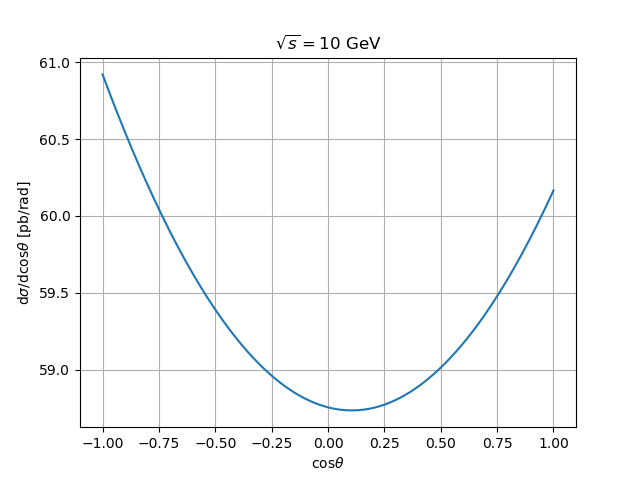
\includegraphics[width=0.45\textwidth]{figures/10gev_diff.png}
}
\subfloat{
	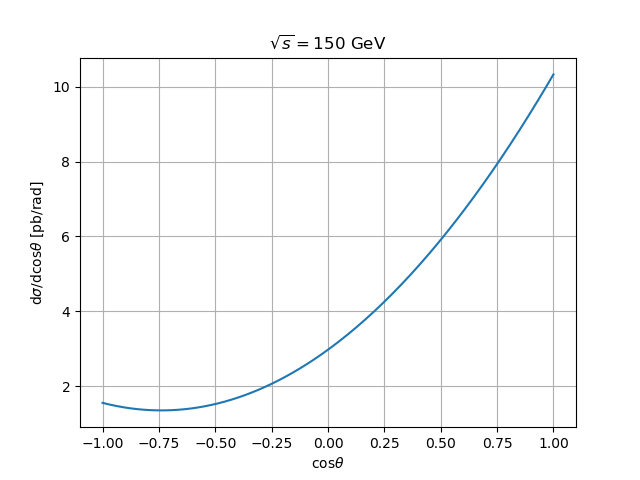
\includegraphics[width=0.45\textwidth]{figures/150gev_diff.png}
}
\caption{differential cross section for $\mu^+\mu^-\rightarrow b\bar{b}$ at $\sqrt{s} = 10$ GeV (a) and  $\sqrt{s} = 150$ GeV (b)}
\label{diffCS}
\end{figure}



\begin{figure}[!ht]
\centering
\subfloat{
	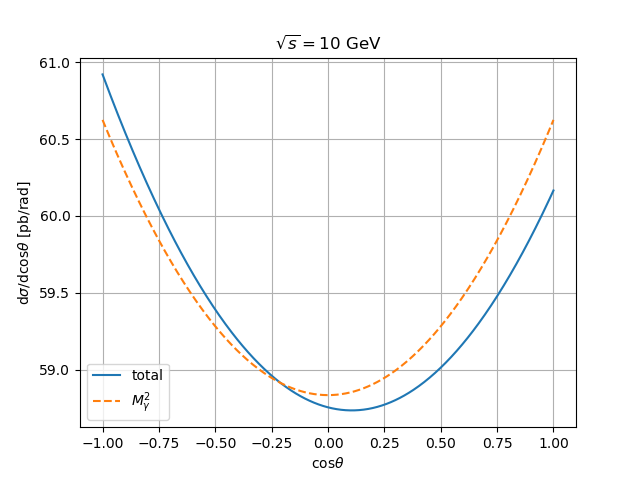
\includegraphics[width=0.45\textwidth]{figures/10gev_diff_A.png}
}
\subfloat{
	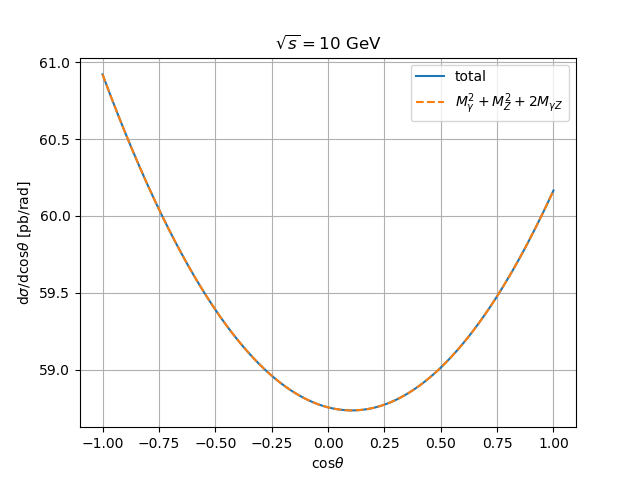
\includegraphics[width=0.45\textwidth]{figures/10gev_diff_AZ.png}
}
\caption{differential cross section for at $\sqrt{s} = 10$ GeV for pure electromagnetic (a) and electroweak (b) process}
\label{150gev_contrib}
\end{figure}

\begin{figure}[!ht]
\centering
\subfloat{
	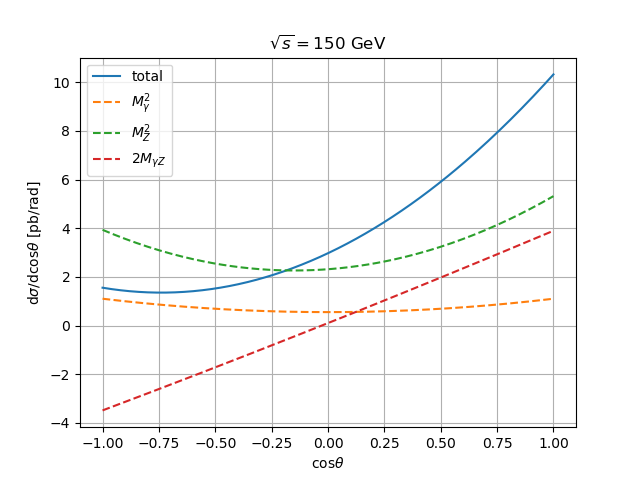
\includegraphics[width=0.45\textwidth]{figures/150gev_diff_terms.png}
}
\subfloat{
	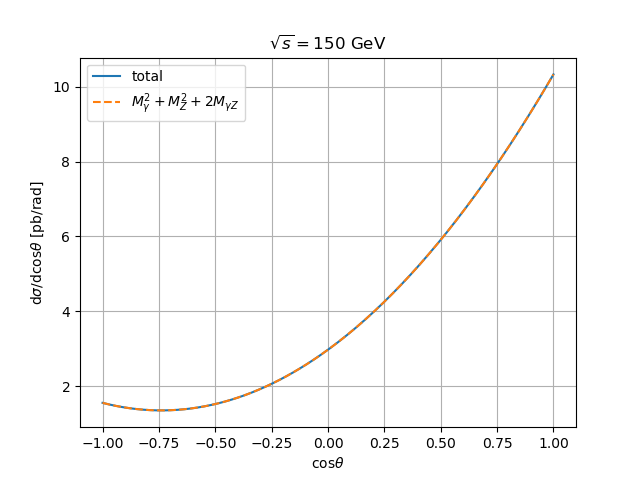
\includegraphics[width=0.45\textwidth]{figures/150gev_diff_ZA.png}
}
\caption{differential cross section for at $\sqrt{s} = 10$ GeV: contribution for each term (a) and electroweak process (b)}
\label{10gev_contrib}
\end{figure}



\begin{figure}[!ht]
\subfloat[pure $\gamma$]{
	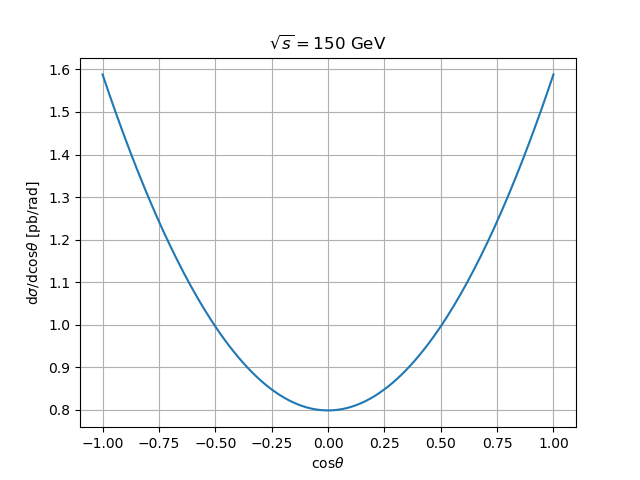
\includegraphics[width=0.33\textwidth]{figures/150gev_termA.png}
}
\subfloat[pure Z]{
	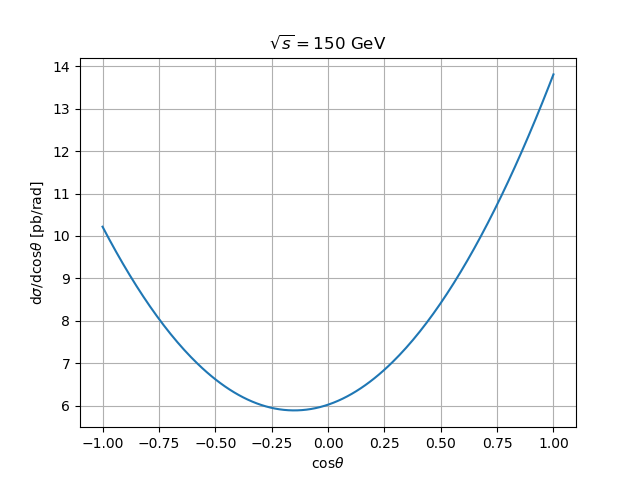
\includegraphics[width=0.33\textwidth]{figures/150gev_termZ.png}
}
\subfloat[pure H]{
	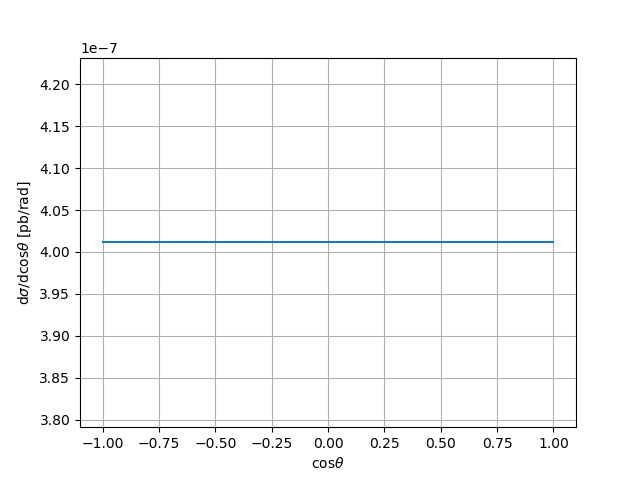
\includegraphics[width=0.33\textwidth]{figures/150gev_termH.png}
}\\
\subfloat[$\gamma Z$ interference]{
	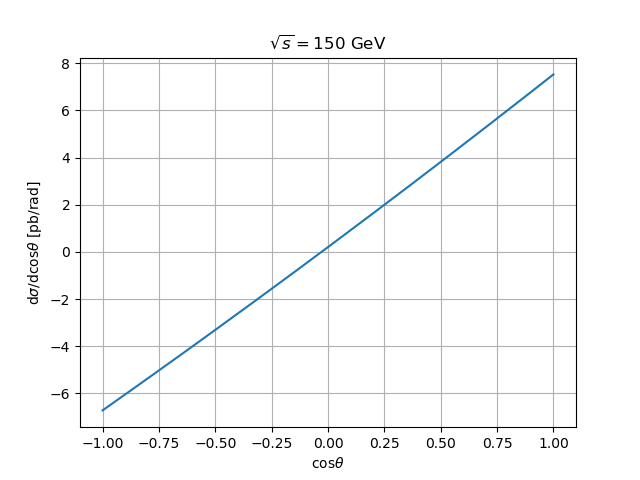
\includegraphics[width=0.33\textwidth]{figures/150gev_termZA.png}
}
\subfloat[$\gamma H$ interference]{
	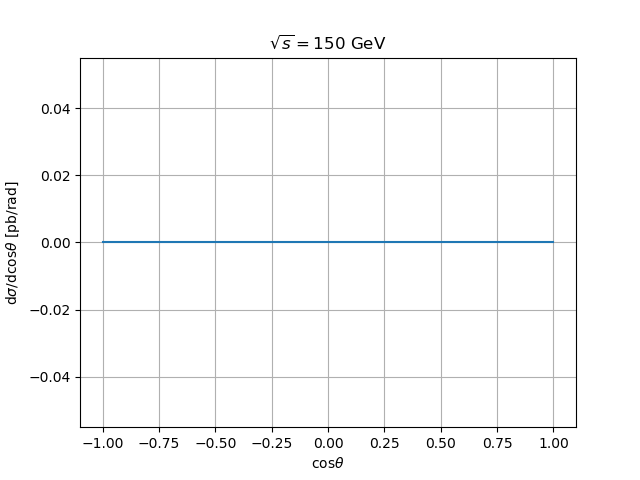
\includegraphics[width=0.33\textwidth]{figures/150gev_termAH.png}
}
\subfloat[$ZH$ interference]{
	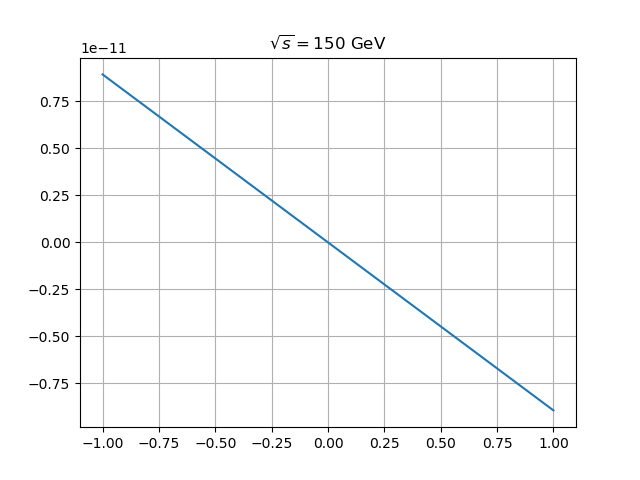
\includegraphics[width=0.33\textwidth]{figures/150gev_termZH.png}
}
\caption{Terms contributing to the differential cross section at $\sqrt{s}=150$ GeV}
\label{150gev_terms}
\end{figure}

% ------------------------------------------------------------------

\subsection{Forward-backward asymmetry}

The forward-backward asymmetry factor is defined as 
\begin{align*}
A_{FB}^l \equiv \frac{\sigma_F - \sigma_B}{\sigma_F+\sigma_B} 
\end{align*}
where $\sigma_F$ and $\sigma_B$ are the differential cross sections $d\sigma/d(\cos\theta)$ integrated respectively from 0 to -1 and from 1 to 0 in $d(\cos\theta)$. It expresses essentially the difference in the couplings of the mediator bosons with right- and left-handed particles. \\
As shown in figure \ref{asymm_terms} (a), the asymmetry for the total amplitude is null at lower energies, where the QED term is dominant, since the differential cross section for a pure QED process is perfectly symmetric.\\
When the energy increases, the cross section for the $Z$ process becomes more and more dominant, thus already at relatively low energies the behaviour of the asymmmetry factor is determined only by the Z couplings.


\begin{figure}[!ht]
\centering
\subfloat[]{
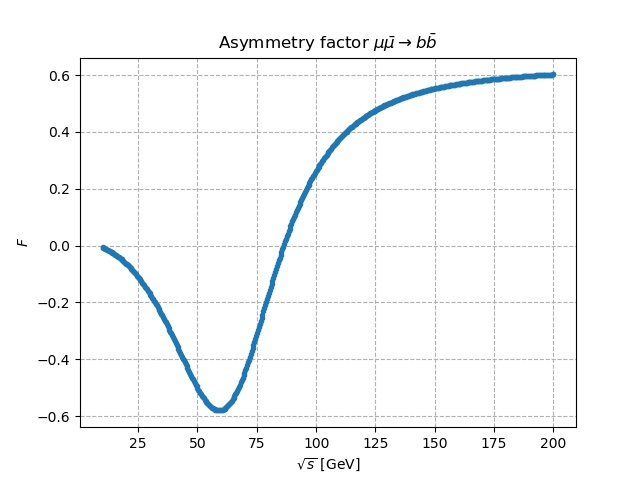
\includegraphics[width=0.45\textwidth]{figures/Asymmetry_tot.jpg}
}
\subfloat[]{
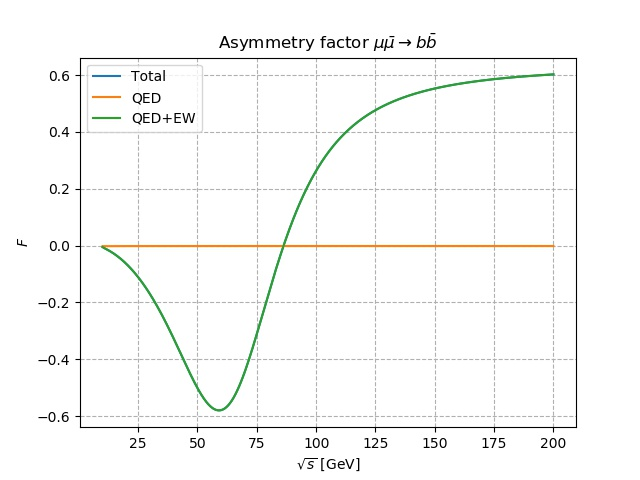
\includegraphics[width=0.45\textwidth]{figures/Asymmetry_terms.jpg}
}
\caption{$\sqrt{s}$ dependence for the asymmetry factor of the process (a) and for the different contributions (b)}
\label{asymm_terms}
\end{figure}

If we consider the asymmetry factor without the $\gamma Z$, we see that the trend is completely different (see figure \ref{asymm_noint}). The sudden drop in the asymmetry factor to negative values is due to the interference effect between $Z$ and $\gamma$, that reaches the minimum when the cross section for QED and Z have the same value (see figure \ref{totalCS_terms}(a)). The trend stabilizes afterwards, when the Z term becomes dominant and interference effects can be neglected.

\begin{figure}[!ht]
\centering
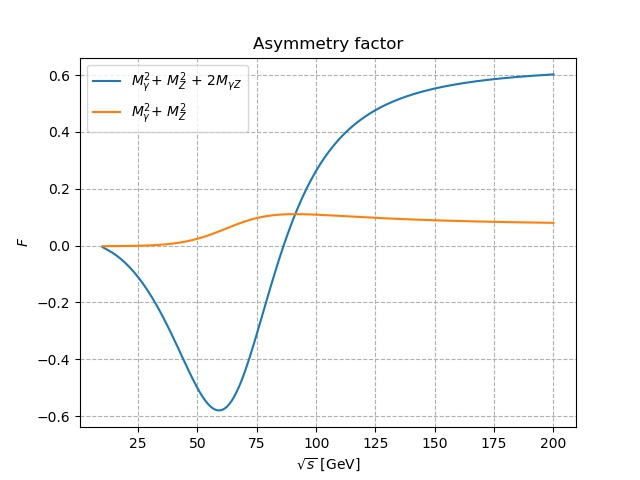
\includegraphics[width=0.6\textwidth]{figures/Asymm_noint.jpg}
\caption{$\sqrt{s}$ dependence of the asymmetry factor with and without $Z\gamma$ interference}
\label{asymm_noint}
\end{figure}

When we compare this process with similar interactions producing other final states, such as $e^+e^-$ and $c\bar{c}$, we immediately note that the asymmetry factor get sharper as the masses of the final states decrease, as shown in figure \ref{asymm_compare}. \\
This is due to the different couplings to LH and RH chiral particle states. Electromagnetism couples to both LH and RH particles, whereas the weak neutral current only couples to doublet isospin states, namely only LH particles and RH antiparticles. The higher the masses, the more our chiral eigenstates are mixed and not coincide to helicity eigenstates; therefore for higher masses we will have a larger number of RH particles that only feel electromagnetism but are blind to the weak interaction. \\
For those particles the symmetry factor will be null because it is the one of a pure QED process, and this effect smoothens the curve of the total process.


\begin{figure}
\centering
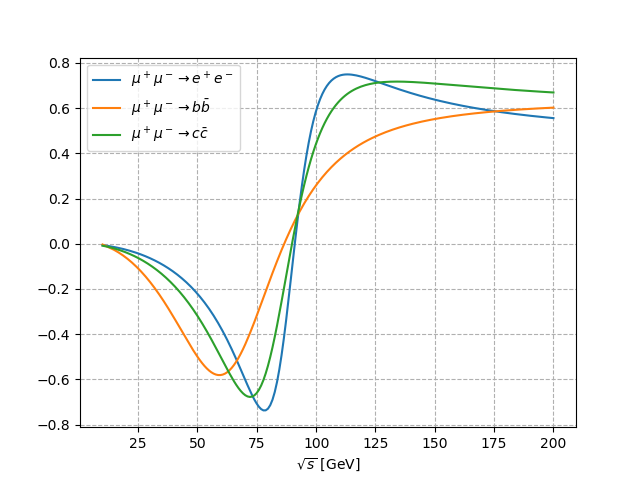
\includegraphics[width=0.6\textwidth]{figures/Compare_asymm.png}
\caption{$\sqrt{s}$ dependence of the asymmetry factor for different final states}
\label{asymm_compare}
\end{figure}

% ------------------------------------------------------------------
% ------------------------------------------------------------------

\section{The total cross section}

The total cross section for the process is shown in figure \ref{totalCS}. 
As expected, it is null under a threshold $\sqrt{s}=2m_{b} = 9.7$ GeV - the energy necessary to produce a $b\bar{b}$ pair - and has a sharp peak for $\sqrt{s}=m_{Z} = 91$ GeV corresponding to the invariant mass of the Z boson. \\
 

\begin{figure}[!ht]
\centering
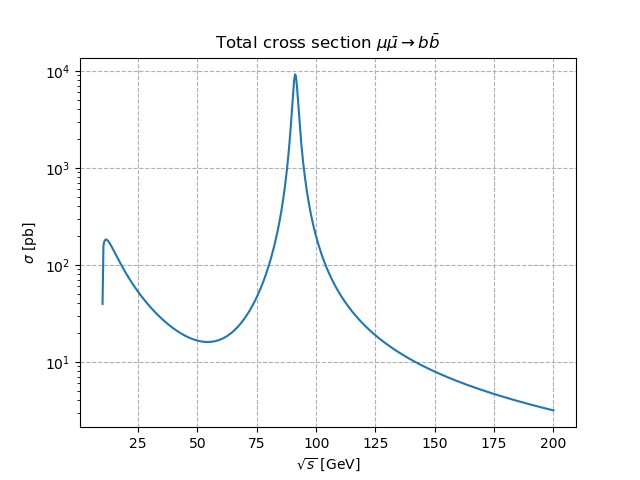
\includegraphics[width=0.6\textwidth]{figures/totalCS.jpg}
\caption{$\sqrt{s}$ dependence for the total cross section of the process }
\label{totalCS}
\end{figure}

If we analyze the single contributions shown in figure \ref{totalCS_terms}, we see that it essentially corresponds to the terms of QED and weak neutral current, whereas the Higgs peak is 2 orders of magnitude smaller than other contributions and cannot be easily resolved. 

\begin{figure}
\centering
\subfloat[]{
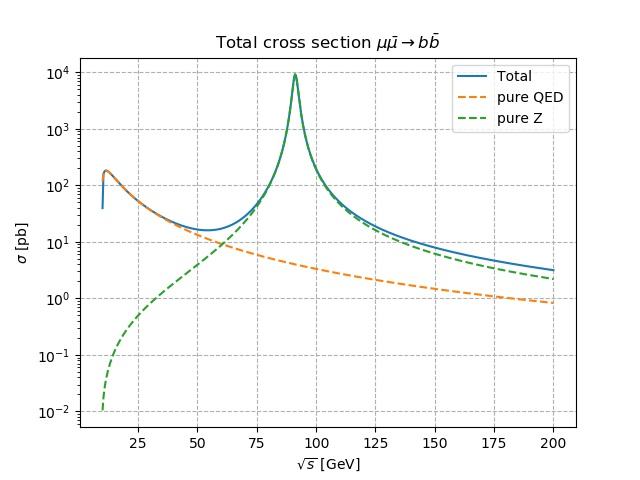
\includegraphics[width=0.45\textwidth]{figures/totalCS_terms.jpg}
}
\subfloat[]{
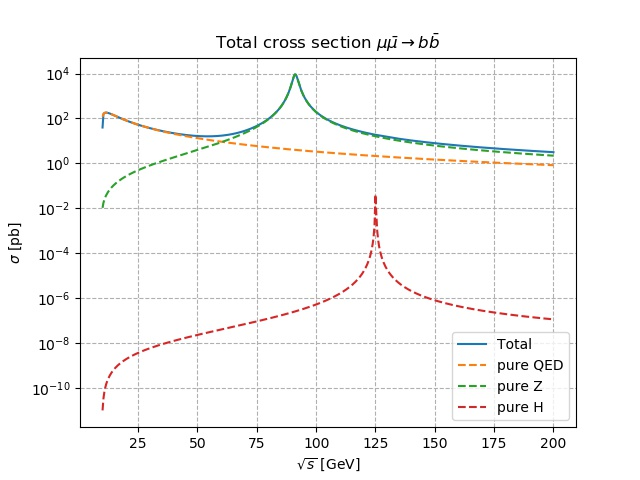
\includegraphics[width=0.45\textwidth]{figures/totalCS_terms_H.jpg}
}
\caption{contributions to the total cross section (a) with pure Higgs term (b)}
\label{totalCS_terms}
\end{figure}


\section{Comparisons with \texttt{CompHEP} simulations}

All the results have been cross-checked with the equivalent events simulated in CompHEP, in particular to spot mistakes in the calculations for the squared amplitude terms. 

\begin{figure}[!ht]
\centering
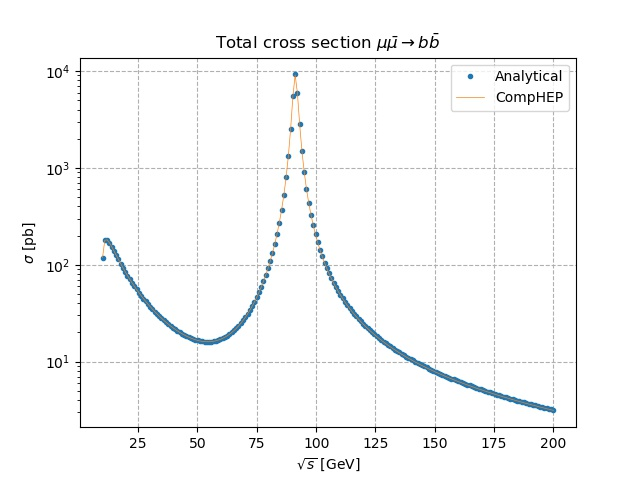
\includegraphics[width=0.6\textwidth]{figures/TotalCS_CH.jpg}
\caption{total cross section - comparison with CompHEP data}
\label{totalCS_ch}
\end{figure}

Figure \ref{totalCS_ch} shows the comparison between the analytical expression for the total cross section and the total cross section obtained in CompHEP.

\begin{figure}
\centering
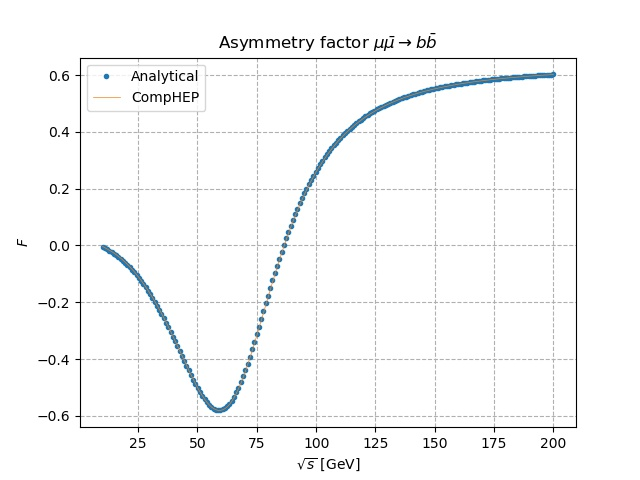
\includegraphics[width=0.6\textwidth]{figures/Asymmetry_CH.jpg}
\caption{asymmetry factor - comparison with CompHEP data}
\label{asymmetry_ch}
\end{figure}

Figure \ref{asymmetry_ch} also shows the comparison between the asymmetry factor simulated from the analytical expression and the one from CompHEP.\\

The CompHEP simulations confirm that the Higgs invariant mass peak cannot be resolved within the considered process and that the results obtained from the analytical expressions are compatible with the Standard Model.

%----------------------------------------------------
%----------------------------------------------------

\section{Adding $Z'$ to the model}

As a further step we add a new boson to the model and use CompHEP to calculate the cross sections for the process $\mu^+\mu^-\rightarrow b\bar{b}$ with this new mediator. 
We assume that it has a much larger mass than the Z, $m_{Z'} = 2.0$ TeV, but for the rest it couples in the same way to fermions and has the same decay width. Note that given the large mass of this particle we have to consider a higher energy range than in the prior tasks.\\

\begin{figure}[!ht]
\centering
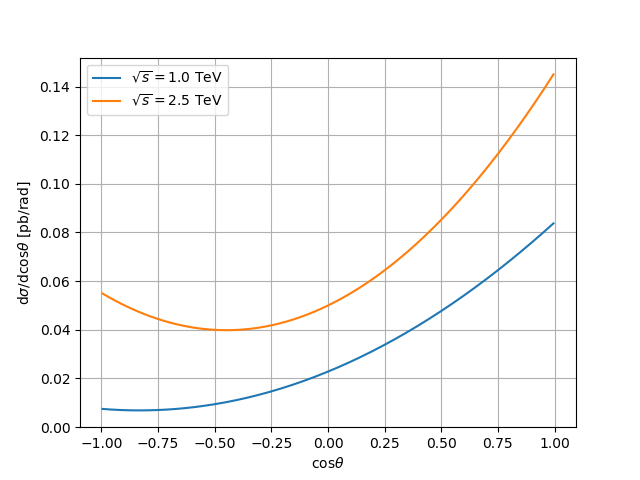
\includegraphics[width=0.6\textwidth]{figures/Zprime_diffCS.png}
\caption{SM with $Z'$, differential cross section for the process}
\label{Z'_diff}
\end{figure}

Figure \ref{Z'_diff} shows the differential cross section at two different values of energies. As expected it is not symmetric because of the different couplings to right- and left-handed particles, and it is higher for the higher energy.\\


This last feature can be understood in terms of the total cross section (see figure \ref{Z'_totalCS}): the two energy values are chosen to be before and after the invariant mass peak. At $1.5$ TeV the cross section has contributions coming from $Z$ and $\gamma$ and the interference effects, and is just starting to feel the effect of $Z'$. At 2.5 GeV though the contribution from Z' are dominant and the other effects have essentially died out, leaving the $\mu^+\mu^-\rightarrow Z'\rightarrow b\bar{b}$ as the only process contributing to the cross section. 

\begin{figure}[!ht]
\centering
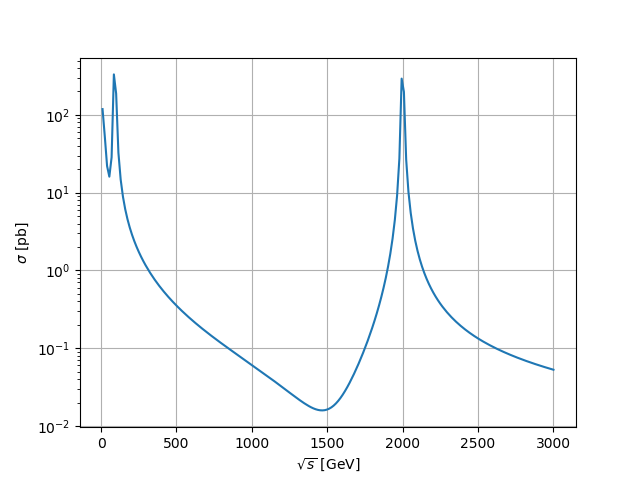
\includegraphics[width=0.6\textwidth]{figures/Zprime_TotalCS.png}
\caption{SM with $Z'$, total cross section for the process}
\label{Z'_totalCS}
\end{figure}

The behaviour of the asymmetry factor (figure \ref{Z'_asymm}) confirms this: after the first minimum due to the $\gamma Z$ interference term the trend becomes stable around the $Z$ contribution, until the next interference with $Z'$ makes it drop again. Afterwards it gets stable to a different value than before, since there is no significant contribution from $Z$ and $\gamma$ anymore. \\

\begin{figure}[!ht]
\centering
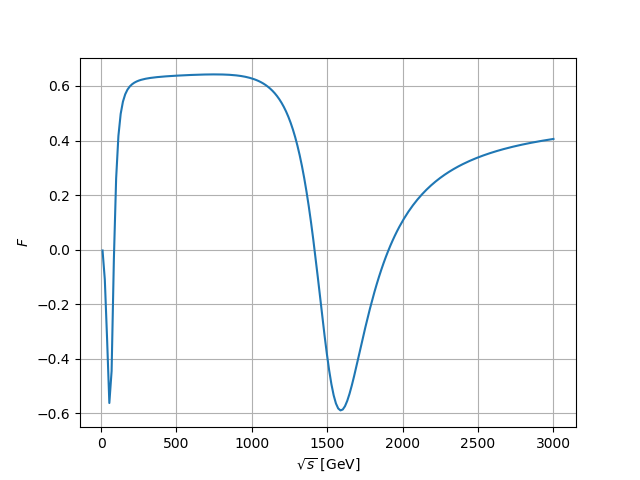
\includegraphics[width=0.6\textwidth]{figures/Zprime_asymm.png}
\caption{SM with $Z'$, asymmetry factor for the process}
\label{Z'_asymm}
\end{figure}

This suggests that a drop in the asymmetry factor, apparing at lower energies than the invariant mass peak itself, is index of the presence of a possibly new particle, and a lower limit for its mass can be set.


%----------------------------------------------------
%----------------------------------------------------


\section{Di-leptons invariant mass from ATLAS}

Following the instructions on Even S. H\aa land's notebook \cite{even} it was possible to access the open data from ATLAS detector at LHC and analyze them using \texttt{ROOT}. 
The process considered is a proton-proton collision with two leptons ($e^+e^-$ or $\mu^+\mu^-$) in the final state:
\begin{align*}
pp \rightarrow l^+l^-\,X\qquad l=e,\mu.
\end{align*}

The invariant-mass distribution for the events is shown in figure \ref{atlas}, and displays the different possible processes leading to two leptons and how frequently they have been detected.

\begin{figure}[!ht]
\centering
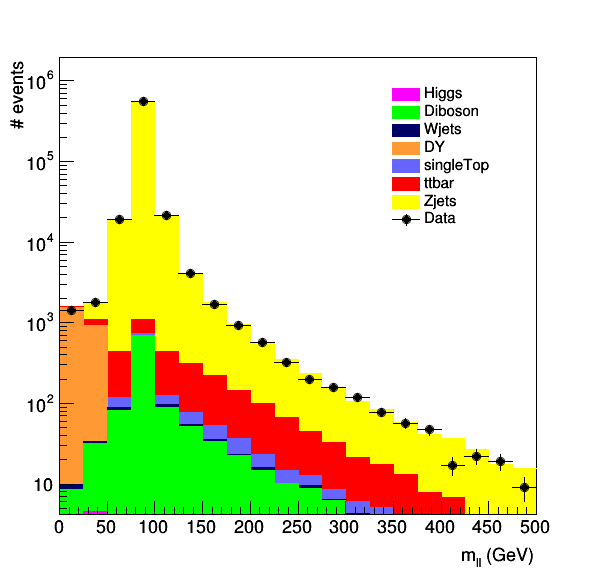
\includegraphics[width=0.6\textwidth]{figures/atlas.jpeg}
\caption{di-lepton invariant mass at ATLAS detector}
\label{atlas}
\end{figure}

At lower energies the main contribution comes from the Drell-Yan process $q\bar{q}\rightarrow l^+l^-$, which fades out rather rapidly in favour of the virtual $Z +$ jets process, which dominates for the rest of the energy scale and shows the invariant mass peak in the bin containing the Z mass value $m_Z = 91$ GeV. Other processes contributing to the background are the $t\bar{t}$ annihilation into a weak Z boson, showing the peak around the same bin, the production of a top quark, two weak bosons, a W and jets. \\
The events corresponding to Higgs production are only 1 out of 1000 at the lowest energy bin, meaning that such a process is not suitable to study the properties of the Higgs due to the great underlying background. 


%----------------------------------------------------
% Thomson

\end{document}
